\documentclass[12pt]{article}
\usepackage[english]{babel}
\usepackage{natbib}
\usepackage[none]{hyphenat}
\usepackage[linktocpage=true]{hyperref}
\usepackage{url}
\usepackage[utf8x]{inputenc}
\usepackage{amsmath}
\usepackage{graphicx}
\usepackage{parskip}
\usepackage{fancyhdr}
\usepackage{vmargin}
\usepackage{color}
\setmarginsrb{3 cm}{2.5 cm}{3 cm}{2.5 cm}{1 cm}{1 cm}{1 cm}{1.5 cm}

\title{Rapport de la tranche 3}							
\author{Nicolas SALLERON\\ Yoann GHIGOFF\\ Kévin VU-SAINTONGE \\ Axel ARCHAMBAULT}							
\date{29 Janvier 2018}									

\makeatletter
\let\thetitle\@title
\let\theauthor\@author
\let\thedate\@date
\makeatother

\pagestyle{fancy}
\fancyhf{}
\rhead{\theauthor}
\lhead{\thetitle}
\cfoot{\thepage}

\begin{document}
%%%%%%%%%%%%%%%%%%%%%%%%%%%%%%%%%%%%%%%%%%%%%%%%%%%%%%%%%%%%%%%%%%%%%%%%%%%%%%%%%%%%%%%%%
\begin{titlepage}
	\centering
    \vspace*{0.5 cm}
    
\includegraphics[scale = 0.10]{UPMC_Sorbonne_Universites_svg.jpg}\\[1.0 cm]	% University Logo
    \textsc{\LARGE Sorbonne université}\\[2.0 cm]	% University Name
	\textsc{\LARGE IDM}\\[0.5 cm]			
	\textsc{\large Les Roboticiens}\\[0.5 cm]				% Course Name
	\rule{\linewidth}{0.2 mm} \\[0.4 cm]
	{ \huge \bfseries \thetitle}\\
	\rule{\linewidth}{0.2 mm} \\[1.5 cm]
	
	\begin{minipage}{0.4\textwidth}
		\begin{flushleft} \large
			\emph{Auteurs:}\\
			\theauthor
			\end{flushleft}
			\end{minipage}~
			\begin{minipage}{0.4\textwidth}
			\begin{flushright} \large
			\emph{Numéros étudiant:} \\
			3504018\\3506454\\3202944\\3300807									% Your Student Number
		\end{flushright}
	\end{minipage}\\[5 cm]
	
	{\large \thedate}\\[2 cm]
 
	\vfill
	
\end{titlepage}
%%%%%%%%%%%%%%%%%%%%%%%%%%%%%%%%%%%%%%%%%%%%%%%%%%%%%%%%%%%%%%%%%%%%%%%%%%%%%%%%%%%%%%%%%
\renewcommand{\contentsname}{Sommaire}
    \tableofcontents
    \newpage

    \section{Introduction}
        La tranche 1 consistait à créer un langage spécifique à la création de chorégraphie pour les drones et à construire un éditeur de texte permettant l'édition et la complétion du langage.
        
        La tranche 2 consistait à transformer la chorégraphie écrite par l'utilisateur en un programme qui sera capable de faire exécuter des commandes au drone en fonction d'une runtime.
        
        La tranche 3 consiste à déployer la solution sur un serveur d'exécution (notre ordinateur ou celui du client) pour tester la distribution réalisée. De plus, une soutenance ou l'équipe présentera des vidéos démontrant la validité de la solution proposée.

    \section{Explication du fonctionnement de la solution}
        Comme expliquée dans le rapport de la Tranche 2, le code écrit par l'utilisateur générera du java qui respectera l'API du drone utilisé (via la Runtime).
        
        Le code de Parrot étant en C, notre code java effectuera un "pont" entre lui-même et un fichier C (créé par nous même) qui communiquera avec l'API de Parrot.
        
        Plus précisément notre code java a pour rôle de :
        
        \begin{itemize}
            \item Créer un flux de sortie en direction de notre programme C.
            \item Créer et gérer les Threads pour la durée des commandes.
        \end{itemize}
    
    \newpage
    \section{Notice d'utilisation}
        Pour commencer, l'utilisateur devra choisir la distribution autonome du produit en fonction du système d'exploitation qu'il utilise pour le démarrer.
        En effet, la distribution est compatible pour les deux OS suivants : MacOS, Linux.
        
        \begin{figure}[!h]
        \centering
        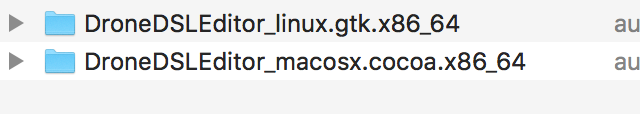
\includegraphics[scale=0.75]{Distrib.png}
        \caption{Versions de la distribution}
        \end{figure}
        
        L'utilisateur devra dézipper l'archive qu'il aura choisi.
        
        Une fois terminé, il aura les fichiers suivants :
        
        
        \begin{figure}[!h]
        \centering
        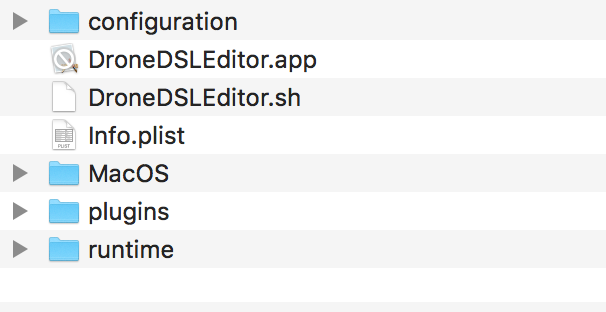
\includegraphics[scale=0.75]{Contenu.png}
        \caption{Fichiers extraits}
        \end{figure}
        
        Il lui suffira de lancer DroneDSLEditor.sh dans un terminal pour pouvoir lancer l'éditeur de création de chorégraphies. \\
        Lors d'une première initialisation, il est nécessaire que l'application récupère et installe des dépendances, il faut donc lancer le script avec l'argument "install". 
        
            \begin{figure}[!h]
         \centering Exemple : “./DroneDSLEditor.sh install"\\
         \end{figure}
        Pour les autres utilisations, cela n'est pas nécessaire et l'utilisateur ne devra taper que : \\
       \begin{figure}[!h]
        \centering “./DroneDSLEditor.sh"\\
        \end{figure}
        \newpage
        Au lancement de l'application il devra spécifier un répertoire pour stocker ses chorégraphies.
        
        \begin{figure}[!h]
        \centering
        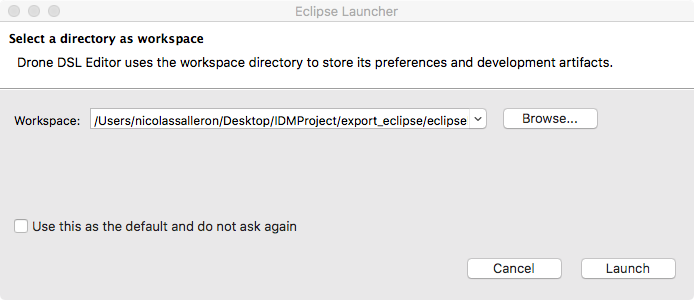
\includegraphics[scale=0.50]{03.png}
        \caption{Répertoire de sauvegarde}
        \end{figure}
        
        Puis il créera un nouveau projet pour qu'il puisse éditer une chorégraphie.
                
        \begin{figure}[!h]
        \centering
        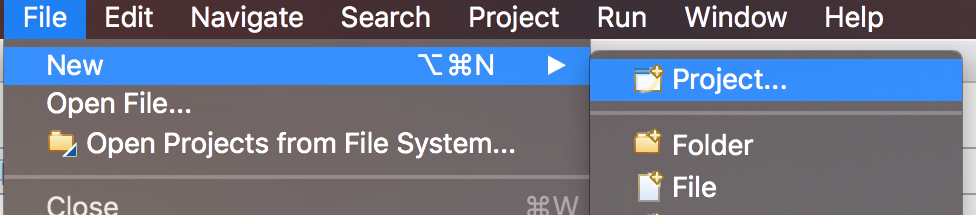
\includegraphics[scale=0.20]{04.png}
        \caption{Nouveau projet}
        \end{figure}
    
        Il devra choisir un projet Xtext nommé DroneDSLProject.
        
        \begin{figure}[!h]
        \centering
        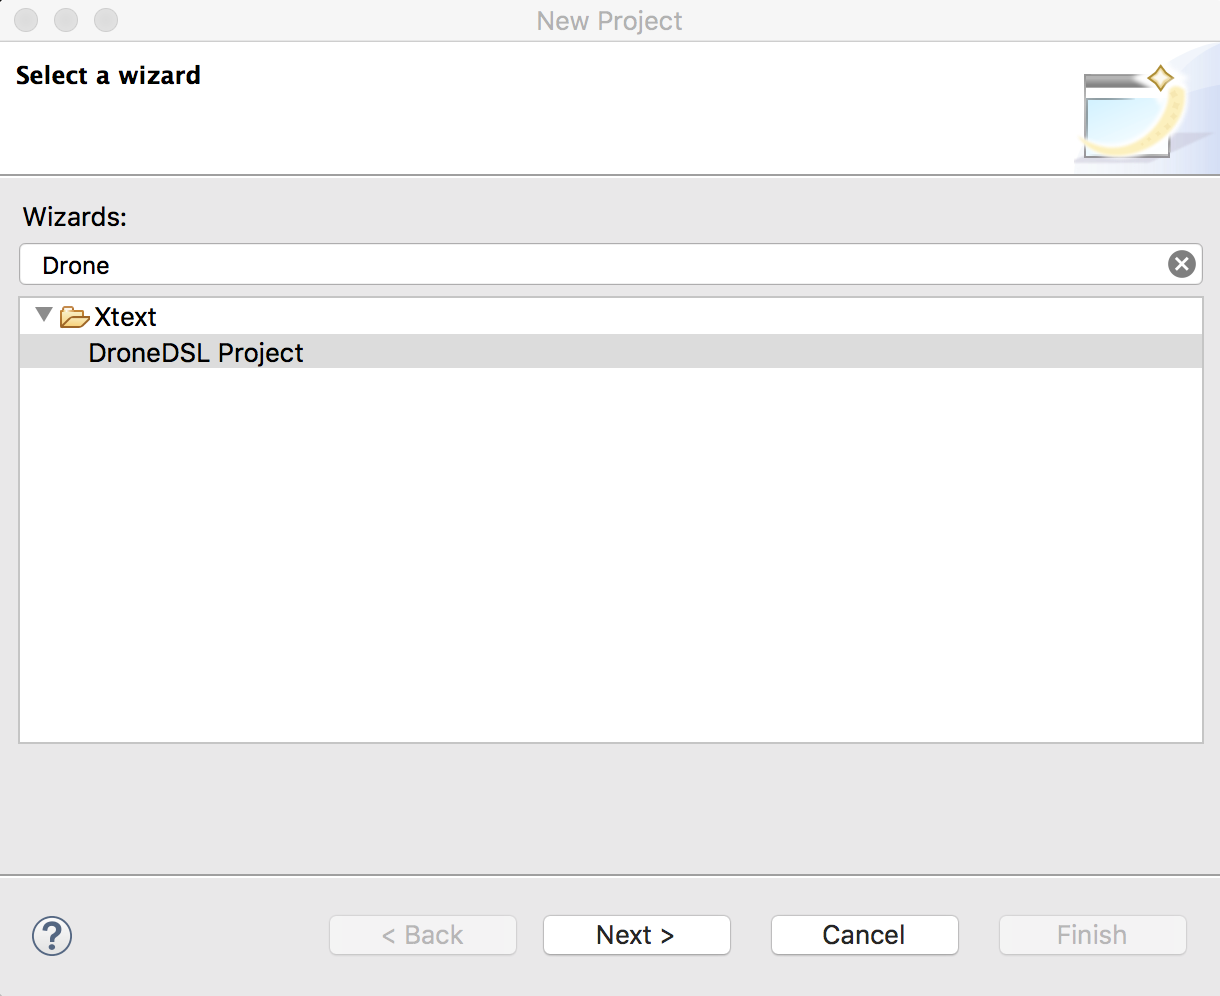
\includegraphics[scale=0.40]{05.png}
        \caption{Nouveau projet}
        \end{figure}
        
        Ensuite l'utilisateur doit nommer son projet.
        
        \begin{figure}[!h]
        \centering
        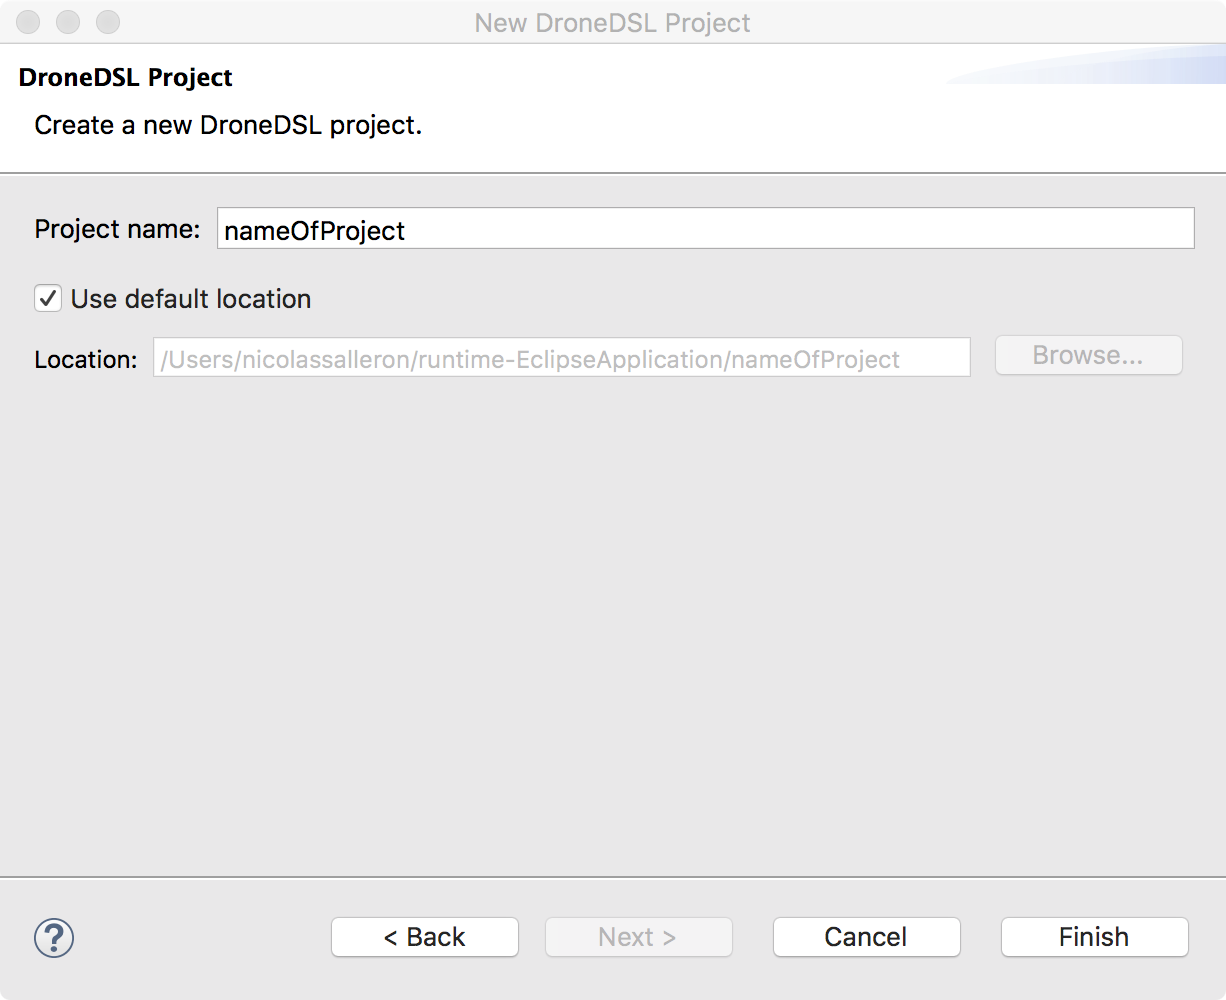
\includegraphics[scale=0.40]{06.png}
        \caption{Nom du projet}
        \end{figure}
        
        \newpage
        Il pourra ainsi créer sa chorégraphie en spécifiant tout d'abord 5 constantes de vol qui sont générées automatiquement. Cela permet au programme d'adapter les instructions. Il définira ainsi la vitesse maximale d'élévation, la vitesse maximale de déplacement, la vitesse maximale de rotation, l'altitude maximale et la distance d'éloignement maximale du drone. Puis il pourra définir le corps main qui représente le point d'entrée du programme. Ce qui est contenu dans le bloc d'instruction suivant ce mot clef sera les instructions exécutées par le drone. Enfin il pourra faire appel à des fonctions définies par l'utilisateur.
        
        \begin{figure}[!h]
        \centering
        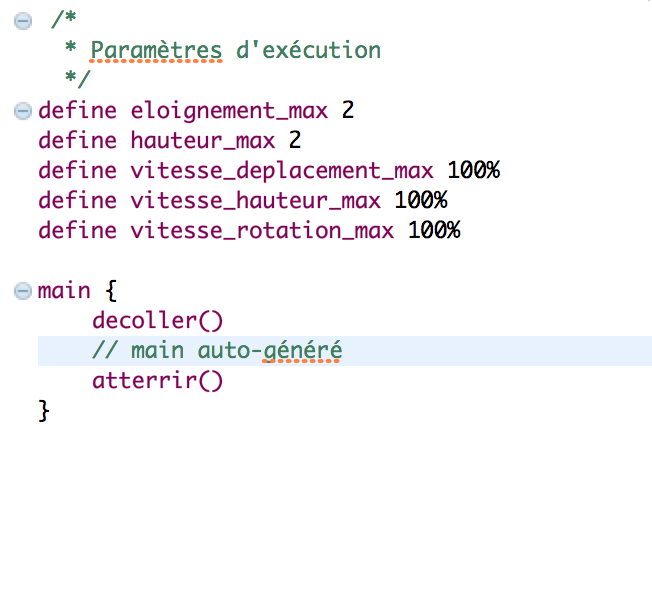
\includegraphics[scale=0.60]{07.png}
        \caption{Exemple de projet}
        \end{figure}
        
        \newpage
        Une fois sa chorégraphie sauvegardée, l'utilisateur doit générer les classes JAVA dont il a besoin pour faire marcher son programme. Pour cela, il cliquera sur le bouton “généré". \textbf{Note : cela doit se faire pour chaque fichier .main\_drone et .lib\_drone (seulement s'ils ont été modifiés). }       
        \begin{figure}[!h]
        \centering
        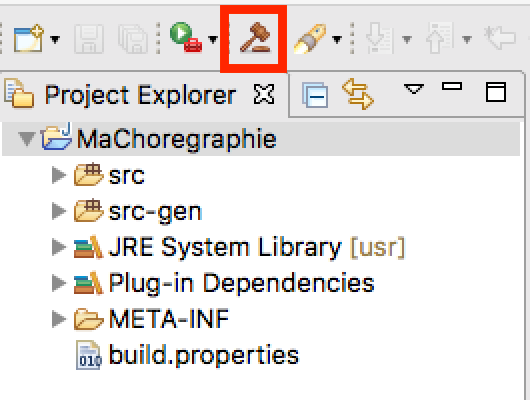
\includegraphics[scale=0.80]{09.png}
        \caption{Structure du projet}
        \end{figure}
        
        Ainsi dans le dossier src du projet on retrouve le fichier main.main\_drone qui représente la chorégraphie définie par l'utilisateur. De plus, les différents packages regroupent les différentes instructions.
        
        L'utilisateur pourra lancer l'exécution de la chorégraphie en sélectionnant le dossier src puis réalisant un click droit, puis run as, puis Java Application. Il pourra également définir un bouton lui permettant d'éviter cette séquence.        
        \begin{figure}[!h]
        \centering
        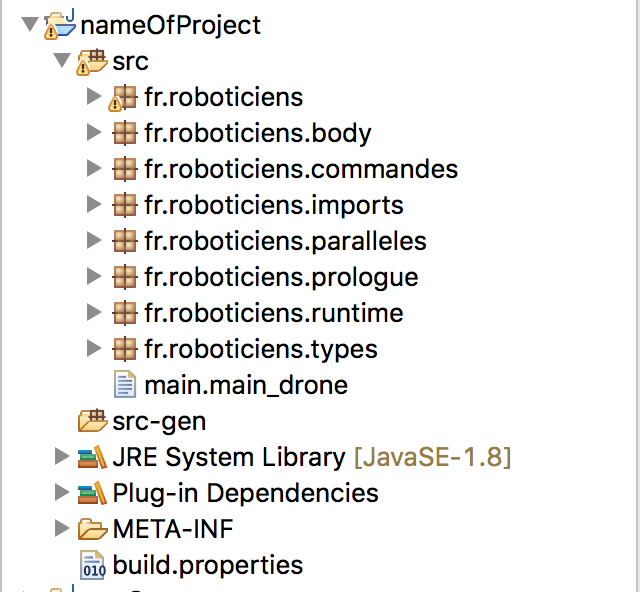
\includegraphics[scale=0.50]{08.png}
        \caption{Structure du projet}
        \end{figure}
        
        \subsection{Langage de conception de chorégraphie}
        		\subsubsection{Prologue}
			Pour fonctionner, l'utilisateur doit définir 5 constantes de vol.
			Cela permet au programme d'adapter la vitesse des mouvements en fonction de ces dernières.
			Il doit les définir comme ceci au début du fichier \newline

			\begin{figure}[h!]
  			      \begin{center}
  			          \begin{verbatim}
   			             define vitesse_hauteur_max 50%
   			             define vitesse_deplacement_max 10%
   			             define vitesse_rotation_max 20%
   			             define hauteur_max 20
   			             define eloignement_max 30
   			         \end{verbatim}
   			     \end{center}
    			    \caption{Exemple de define}
    			    \label{Exemple de define}
   			 \end{figure}

			\paragraph{}\textbf{define vitesse\_hauteur\_max 100\%: } \\
				Cette constante permet de définir la vitesse maximale d'élévation du drone pour la chorégraphie par rapport à sa vitesse maximale possible. \newline
				La valeur de cette constante doit être comprise entre 1 et 100\%.
			\paragraph{}\textbf{define vitesse\_deplacement\_max 100\%:}\\
				Cette constante permet de définir la vitesse maximale de déplacement sur le plan horizontal du drone pour la chorégraphie par rapport à sa vitesse maximale possible. \newline
				La valeur de cette constante doit être comprise entre 1 et 100\%.
			\paragraph{}\textbf{define vitesse\_rotation\_max 100\% :}\\
				Cette constante permet de définir la vitesse maximale de rotation du drone pour la chorégraphie par rapport à sa vitesse maximale. \newline
				La valeur de cette constante doit être comprise entre 1 et 100\%.
			\paragraph{}\textbf{define hauteur\_max 150 :}\\
				Cette constante permet de limiter l'altitude maximale du drone en vol. Lorsque le drone est sur le point de dépasser cette limite, il se stabilise automatiquement à la hauteur maximale. \newline
				La valeur de cette constante doit être un entier positif qui ne doit pas être supérieure à la hauteur maximale possible du drone.
			\paragraph{}\textbf{define eloignement\_max 3000:}\\
				Cette constante permet de contrôler la distance horizontale du drone en vol. Lorsque le drone est sur le point de dépasser cette limite, il se stabilise automatiquement à la distance maximale horizontale. \newline
				La valeur de cette constante doit être un entier positif qui ne doit pas être supérieure à la distance maximale horizontale possible du drone.

        \subsubsection{Les types}
      	\paragraph{}Type "Pourcent":\\
		Déclaration : Pourcent a = 10\%\\
		C'est le type utilisé pour en paramètre des commandes de déplacement (monter, descendre, gauche, droite, avancer, reculer, rotation\_gauche, rotation\_droite).\\
		La valeur doit être comprise entre 1 et 100
	\paragraph{}Type "Seconde": \\ 
		Déclaration : Seconde b = 10\\
		C'est le type utilisé pour en paramètre des commandes de déplacement (monter, descendre, gauche, droite, avancer, reculer, rotation\_gauche, rotation\_droite).\\
	\subsubsection{Décollage}
		\quad Syntaxe: \textbf{decoller()}\bigbreak
			Cette commande permet à un drone de décoller. Elle devra obligatoirement être la première commande exécutée dans le bloc main et ne peut pas être à nouveau exécutée si le drone n'a pas atterri.\\
			Il est uniquement possible de décoller si le drone est au sol. 
	\subsubsection{Attérrissage}

		\quad Syntaxe: \textbf{atterrir()}\bigbreak
			Cette commande permet à un drone d'atterrir. Elle devra obligatoirement être la dernière commande exécutée dans le bloc main et ne peut pas être à nouveau exécutée si le drone n'a pas décoller. \\
			Il est uniquement possible d'atterrir si le drone est en vol.

	\subsubsection{Les commandes de mouvements}

		\quad Syntaxe: \textbf{monter(durée: Seconde, vitesse\_verticale: Pourcent)} \bigbreak
			Cette commande permet à un drone de monter en altitude. \\
			Elle ne peut être exécutée que si le drone est en vol. \\
			Le paramètre \textbf{durée} est le temps en type Seconde durant lequel le drone s'élève. \\
			Le paramètre \textbf{vitesse\_vertical} est un type Pourcent. Il indique la vitesse d'élévation du drone par rapport à la vitesse verticale maximum définie par l'utilisateur dans le prologue. \\

		\quad Syntaxe: \textbf{descendre(durée: Seconde, vitesse\_verticale: Pourcent)} \bigbreak
			Cette commande permet à un drone de descendre en altitude. \\
			Elle ne peut être exécutée que si le drone est en vol.\\
			Le paramètre \textbf{durée} est le temps en type Seconde durant lequel le drone s'élève. \\
			Le paramètre \textbf{vitesse\_vertical} est un type Pourcent. Il indique la vitesse d'élévation du drone par rapport à la vitesse verticale maximum définie par l'utilisateur dans le prologue. \\

		
		\quad Syntaxe: \textbf{avancer(durée: Seconde, vitesse\_deplacement: Pourcent)}  \bigbreak
			Cette commande permet à un drone de se déplacer sur un axe horizontal dans la direction vers laquelle sa face avant est tournée. \\
			Elle ne peut être exécutée que si le drone est en vol.\\
			Le paramètre \textbf{durée} est le temps en type Seconde durant lequel le drone avance. \\
			Le paramètre \textbf{vitesse\_deplacement} est un type Pourcent. Il indique la vitesse de déplacement du drone par rapport à la vitesse horizontale maximum définie par l'utilisateur dans le prologue.  \\


		\quad Syntaxe: \textbf{reculer(durée: Seconde, vitesse\_deplacement: Pourcent))}  \bigbreak
			Cette commande permet à un drone de se déplacer sur un axe horizontal dans la direction opposée à celle vers laquelle est tournée sa face avant. \\
			Elle ne peut être exécutée que si le drone est en vol.\\
			Le paramètre \textbf{durée} est le temps en type Seconde durant lequel le drone recule. \\
			Le paramètre \textbf{vitesse\_deplacement} est un type Pourcent. Il indique la vitesse de déplacement du drone par rapport à la vitesse horizontale maximum définie par l'utilisateur dans le prologue.  \\


		\quad Syntaxe: \textbf{gauche(durée: Seconde, vitesse\_deplacement: Pourcent))}  \bigbreak
			Cette commande permet à un drone de se déplacer sur un axe horizontal dans la direction à gauche de celle vers laquelle est tournée sa face avant.  \\
			Elle ne peut être exécutée que si le drone est en vol. \\
			Le paramètre \textbf{durée} est le temps en type Seconde durant lequel le drone se déplace. \\
			Le paramètre \textbf{vitesse\_deplacement} est un type Pourcent. Il indique la vitesse de déplacement du drone par rapport à la vitesse horizontale maximum définie par l'utilisateur dans le prologue.  \\

		\quad Syntaxe: \textbf{droite(durée: Seconde, vitesse\_deplacement: Pourcent))}  \bigbreak
			Cette commande permet à un drone de se déplacer sur un axe horizontal dans la direction à droite de celle vers laquelle est tournée sa face avant. \\
			Elle ne peut être exécutée que si le drone est en vol.\\
			Le paramètre \textbf{durée} est le temps en type Seconde durant lequel le drone se déplace. \\
			Le paramètre \textbf{vitesse\_deplacement} est un type Pourcent. Il indique la vitesse de déplacement du drone par rapport à la vitesse horizontale maximum définie par l'utilisateur dans le prologue.  \\

		\quad Syntaxe: \textbf{rotation\_gauche(durée: Seconde, vitesse\_rotation: Pourcent)}  \bigbreak
			Cette commande permet à un drone de tourner sur lui même dans le sens inverse des aiguilles d'une montre. \\
			Elle ne peut être exécutée que si le drone est en vol.\\
			Le paramètre \textbf{durée} est le temps en type Seconde durant lequel le drone doit pivoter.\\
			Le paramètre \textbf{vitesse\_rotation} est un type Pourcent. Il indique la vitesse de déplacement du drone par rapport à la vitesse de rotation maximum définie par l'utilisateur dans le prologue.  \\


		\quad Syntaxe: \textbf{rotation\_droite(durée: Seconde, vitesse\_rotation: Pourcent)}  \bigbreak
			Cette commande permet à un drone de tourner sur lui même dans le sens des aiguilles d'une montre.\\ 
			Elle ne peut être exécutée que si le drone est en vol.\\
			Le paramètre \textbf{durée} est le temps en type Seconde durant lequel le drone doit pivoter.\\
			Le paramètre \textbf{vitesse\_rotation} est un type Pourcent. Il indique la vitesse de déplacement du drone par rapport à la vitesse de rotation maximum définie par l'utilisateur dans le prologue.  \\

	\subsubsection{La commande pause}
		\quad Syntaxe: \textbf{pause(durée: Seconde)}  \bigbreak
			Cette commande permet à un drone de s'arrêter en position stationnaire pendant une certaine durée, soit en vol ou au sol. \\
			Le paramètre \textbf{durée} donnera le temps en secondes durant lequel le drone doit se stabiliser. \\
	
\subsection{Les fonctions}
Le langage permet de définir des fonctions, ces dernières sont une suite d'instructions séquentielles qu'exécutera le drone.\\
Les fonctions ont un nom qui permet de les identifier.
Il n'est pas possible de paralléliser deux fonctions.\\
La définition d'une fonction est de la forme suivante :

    \begin{figure}[h!]
        \begin{center}
            \begin{verbatim}
            func nomDeLaFonction() {
                Mettre une instruction par ligne
            }
            \end{verbatim}
        \end{center}
        \caption{Exemple de definition de fonction}
        \label{Exemple de definition de fonction}
    \end{figure}
    
Il n'est pas possible de réaliser des récursions de fonction. 
	\subsubsection{Fonctions locales}
	
	Les fonctions locales sont des fonctions définies dans le même fichier que le bloc main (fichier d'extension .main\_drone). \\
	L'appel d'une fonction locale se fait sans précision du nom du fichier dans lequel elle est définie.
	
    \begin{figure}[h!]
        \begin{center}
            \begin{verbatim}
            main {
                decoller()
                gauche(1,10%)
                maFonction()
                reculer(1,20%)
                atterrir()
            }
                
            func maFonction() {
                monter(2,10%) & droite(1,15%)
                avancer(2,20%)
                droite(2,15%)
            }
            
            \end{verbatim}
        \end{center}
        \caption{Exemple d'appel d'une fonction locale}
        \label{Exemple d'appel d'une fonction locale}
    \end{figure}

	
	\subsubsection{Bibliothèque de fonction}

	Il est possible d'utiliser des fonctions définies dans d'autres fichiers .lib\_drone, ces fichiers doivent être dans le même répertoire que le fichier appelant ses fonctions.\\
	L'inclusion d'une bibliothèque se fait en définissant via l'instruction \textbf{import} suivi du nom du fichier suivi de l'extension ".lib\_drone".\\
	L'appel d'une fonction définie dans une bibliothèque se fait en précisant le nom du fichier contenant sa définition.\\
	
	  \begin{figure}[h!]
       		 \begin{center}
        		    \begin{verbatim}
		             /* import du fichier contenant la fonction maFonction() */
		             import <maLib.lib_drone>	
		             /* Instructions de prologue */
		             main {
		                decoller()
		                maLib.maFonction()
		                atterrir()
		             }
        		    \end{verbatim}
        		\end{center}
   	 \end{figure}
	
	\newpage
	Fichier maLib.lib\_drone : \\
   	\begin{figure}[h!]
       		 \begin{center}
            		\begin{verbatim}
		             func maFonction() {
		                monter(2,10%) & droite(1,15%)
		                avancer(2,20%)
		                droite(2,15%)
		             }
           		 \end{verbatim}
        		\end{center}
   	 \end{figure}
   	 
   	 \section{Fonctionnement de la distribution}
   	    
   	    La distribution génère un programme JAVA. Ce dernier communique avec le programme C qui appelle les fonctionnalités de l'API du drone fournies par le SDK de Parrot.
   	    
   	    Ainsi lorsque l'utilisateur entre une commande pour sa chorégraphie, elle appelle la commande execute de la classe JAVA associée à la commande. En fonction de la runtime (il y en a une par API de drone) passée en paramètre, la méthode fait appel au code C de Parrot.
   	    
   	    De plus comme nous avons choisi d'associer une durée à une commande, nous avons décidé d'utiliser les Threads. Ces derniers nous permettent pour les instructions basiques d'attendre la fin d'une commande avant d'en exécuter une autre par le drone. Pour les commandes parallélisables, chaque commande est associée à un Thread et est lancée sans attendre la fin de la précédente.
   	    
   	    En résumé :
   	    \begin{itemize}
    \item Chorégraphie écrite par l'utilisateur.
	\item Chorégraphie interprétée et compilée pour générer des classes JAVA (dont la principale nommée Main).
    \item La classe Main créer les classes représentant les mouvements que doit faire le drone.
    \item Le JAVA ouvrira un flux en direction de notre programme C.
    \item Chacune de ces classes utilisent la runtime pour envoyer des informations à ce programme C.
    \item Le C interprète ces informations et envoit des commandes au drone via l'API du constructeur.
	\end{itemize}
        
\end{document}